%%%%%%%%%%%%%%%%%%%%%%%%%%%%%%%%%%%%%%%%%%%%%%%%%%%%%%%%%% 
\chapter{グラフ彩色問題とその関連問題}
%%%%%%%%%%%%%%%%%%%%%%%%%%%%%%%%%%%%%%%%%%%%%%%%%%%%%%%%%%

%%%%%%%%%%%%%%%%%%%%%%%%%%%%%%%%%
\begin{figure}[tb]
  \begin{tabular}{cc}
    \begin{minipage}[t]{0.45\linewidth}
      \centering
      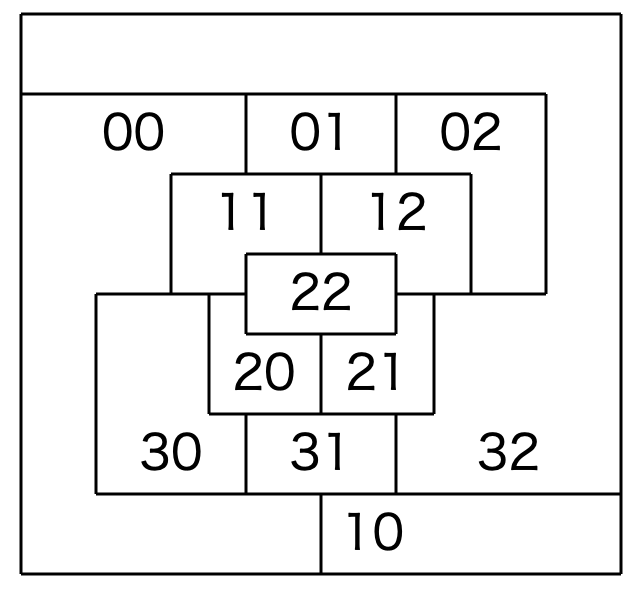
\includegraphics[keepaspectratio,clip,scale=0.2]{fig/order3.png}
      \caption{~\code{order}3の~\code{McGregor}~グラフ}
      \label{fig:order3}
    \end{minipage}
    \begin{minipage}[t]{0.45\linewidth}
      \centering
      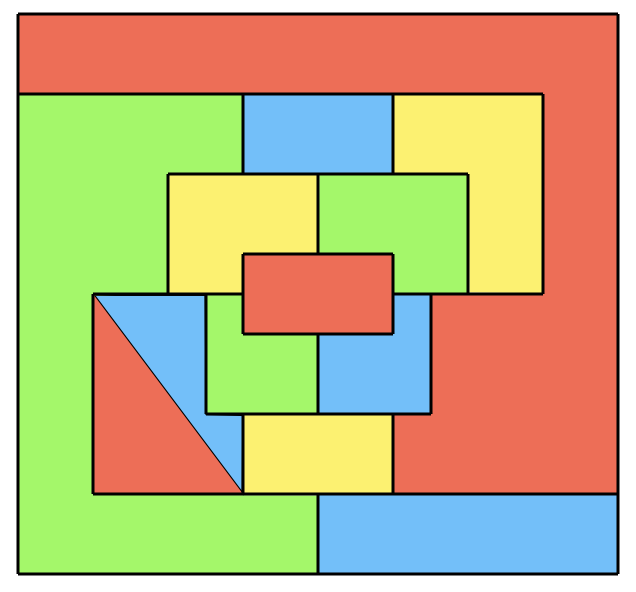
\includegraphics[keepaspectratio,clip,scale=0.2]{fig/order3_mult.png}
      \caption{多色頂点数最大化問題の解の一例}
      \label{fig:order3mult}
    \end{minipage}
  \end{tabular}
\end{figure}
%%%%%%%%%%%%%%%%%%%%%%%%%%%%%%%%%

グラフの各頂点を隣接する頂点と異なる色で彩色することを
\textbf{グラフ彩色問題(Graph Coloring)}もしくは
\textbf{グラフ点彩色問題}と呼ぶ.
以下に本論文で対象となる問題群について述べる.

\begin{itemize}
\item \textbf{グラフ彩色判定問題}は
  与えられたグラフと色数に対してグラフ点彩色が可能かどうかを判定する問題である.
\item \textbf{グラフ彩色における同色頂点数最小化問題}は
  グラフ彩色問題において,同色で彩色する頂点数を最小化する問題である.
\item \textbf{グラフ彩色における同色頂点数最大化問題}は
  グラフ彩色問題において,同色で彩色する頂点数を最大化する問題である.
\item \textbf{グラフ彩色における多色頂点数最大化問題}は
  グラフ彩色問題において,2色以上で彩色できる頂点数を最大化する問題である.
\end{itemize}

図~\ref{fig:order3}は,D.~E~.Knuthの教科書
The Art of Computer Programming~\cite{Knuth:TAOCP:SAT}
に記載されている~\code{order}~3の~\code{McGregor}~グラフである.
このグラフは,頂点数が12で辺数が30のグラフであり,
各頂点には00から32までの頂点番号が振られている.
次に,図~\ref{fig:order3mult}に図~\ref{fig:order3}における,
グラフ彩色における多色頂点数最大化問題の解の一例を示す.
図~\ref{fig:order3mult}は,
赤と青で彩色されている頂点番号30のみ多色で彩色できることを表している.
したがって,図~\ref{fig:order3mult}の
グラフ彩色における多色頂点数最大化問題の解は1である.
また,図~\ref{fig:order3mult}は図~\ref{fig:order3}の
グラフ彩色問題の解の2つを圧縮して表している.
このように,グラフ彩色における多色頂点数最大化問題により,得られた解は,
グラフ彩色問題の解の一部を圧縮した形の解が得られる.


%%% Local Variables:
%%% mode: latex
%%% TeX-master: "paper"
%%% End:
